%
% Szakdolgozatminta az Eszterházy Károly Katolikus Egyetem
% matematika illetve informatika szakos hallgatóinak.
%

\documentclass[
% opciók nélkül: egyoldalas nyomtatás, elektronikus verzió
% twoside,     % kétoldalas nyomtatás
% tocnopagenum,% oldalszámozás a tartalomjegyzék után kezdődik
]{thesis-ekf}
\usepackage[T1]{fontenc}
\PassOptionsToPackage{defaults=hu-min}{magyar.ldf}
\usepackage[magyar]{babel}
\usepackage{mathtools,amssymb,amsthm,pdfpages}
\footnotestyle{rule=fourth}

\newtheorem{tetel}{Tétel}[chapter]
\theoremstyle{definition}
\newtheorem{definicio}[tetel]{Definíció}
\theoremstyle{remark}
\newtheorem{megjegyzes}[tetel]{Megjegyzés}

\begin{document}

\institute{Matematikai és Informatikai Intézet}
\title{Mesterséges intelligencia számítógépes játékokban}
\author{Herbák Marcell\\Programtervező Informatikus BSc}
\supervisor{Dr. Kovásznai Gergely\\Egyetemi docens}
\city{Eger}
\date{2025}
\maketitle

\tableofcontents

\chapter{Bevezetés}

\section{Játék ismertetése}

\begin{figure}[h!]
	\centering
	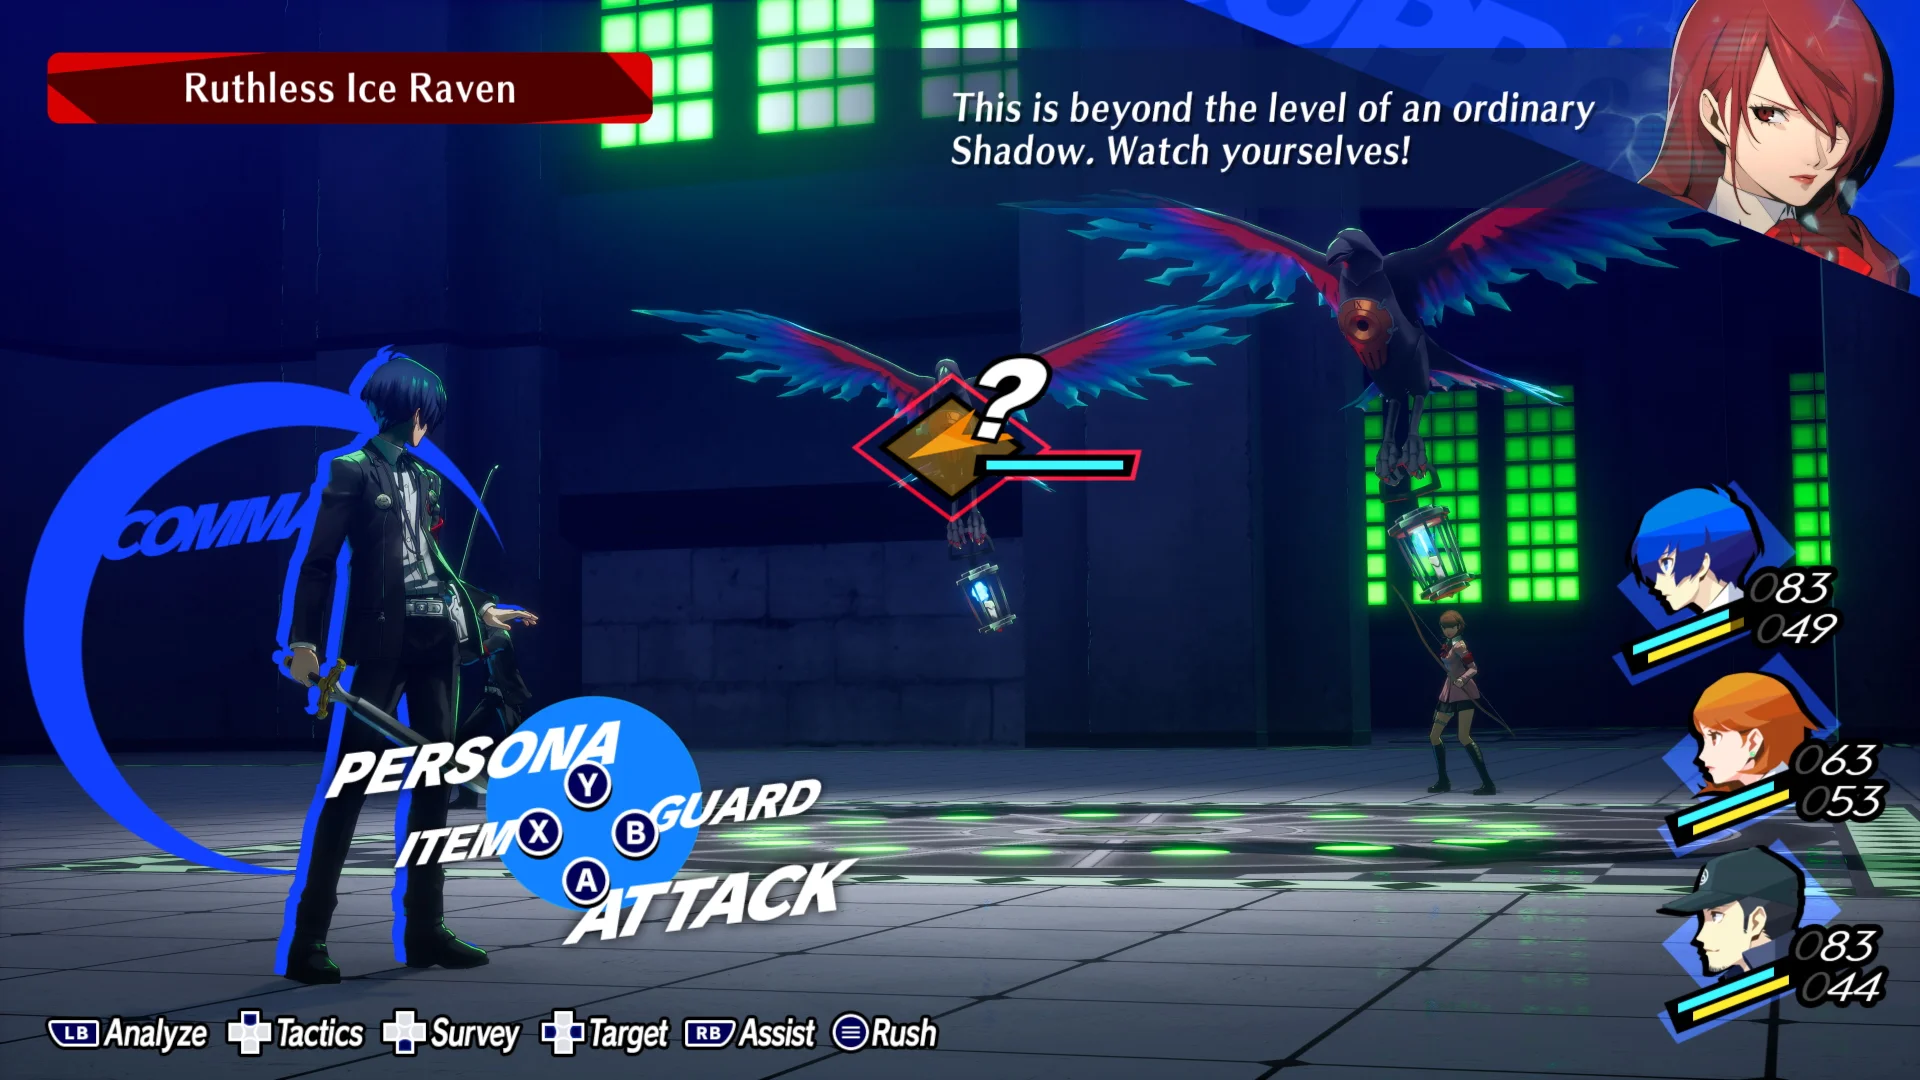
\includegraphics[width=14cm]{./pictures/persona3_xbox.png}
	\caption{Persona 3 Reload}
	\label{persona3}
\end{figure}

\subsection{Játék ötlete}

Szakdolgozatom programjaként egy olyan játékot szerettem volna készíteni, amely nem csak jól implementálható, hanem amivel szabadidőmet is szívesen töltöm. Választásom végül is egy körökre osztott stratégiai játék elkészítésére esett. Ötletadónak, az általam kedvelt videójáték szériát, a Persona játékokat választottam. Az első Persona játék közel 30 éve jelent meg a Shin Megami Tensei szériának spin--off-jaként, így a játékok működésben és történetben bár eltérőek a modern megjelenésektől, jelenleg legfrissebb 2024-ben kiadott (\ref{persona3} ábra) Persona 3 Reload-tól, a játék fő mechanikája nem változott: a játékos karakterei csatába kerülnek egy fix számú, hasonló képességű ellenfelekkel szembe. Ezekben a játékokban, különleges képességekkel rendelkező, úgynevezett Personákkal harcolnak a különböző szereplők.\cite{Persona,Persona3}

Bár a modern játékokban nem alkalmazzák már, a Revelations: Persona harcrendszere (\ref{persona1} ábra) rendelkezett mezőkre felbontott csatatérrel, amelyeknél még a támadásoknak volt egy bizonyos maximális távolsága. Ezek alapján szerettem volna egy olyan játékteret készíteni, ahol a játékosnak nem csak a támadásának a távolságát kell figyelembe vennie, hanem a helyét is a csatatéren. \cite{Persona1,Persona1Gameplay}
\begin{figure}[h!]
	\centering
	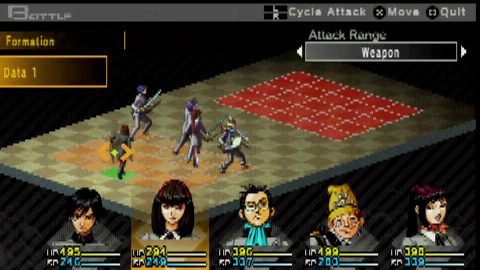
\includegraphics[width=13cm]{./pictures/persona_psp.png}
	\caption{Revelations: Persona}
	\label{persona1}
\end{figure}

\subsection{Játék szabályok} \label{rules}

A játék egy fixált méretű, négyzetekből álló, 7x10 nagyságú táblán folyik. A játékot kettő játékos tudja játszani, melyből a szakdolgozatomban az egyik játékos a mesterséges intelligencia lesz. Mindegyik játékos rendelkezik karakterekkel, amelynek kezdő mennyisége a játék indítása előtt kiválasztható. Mindkét játékos rendelkezik minimum 1, maximum pedig 3 karakterrel. A karakterek mennyisége játékosonként eltérő lehet, nem szükséges mindkét játékosnak ugyanazzal a karakter mennyiséggel kezdenie. Az egyik játékos karakterei (több karakter esetén függőlegesen egy mező kihagyással) a 2. oszlopban, a másik játékos karakterei pedig a 9. oszlopban kezdenek. A táblán léteznek akadályozó mezők, amelyekre a játékosok nem léphetnek, illetve nem támadhatják meg. 

A játék során a játékosok egymás után jönnek, egy körben az összes karakterükkel végre kell hajtaniuk egy interakciót. Ez a két interakció \emph{lépés} és \emph{támadás} lehet. Lépés során a karakterükkel egy mezőt léphetnek a négy irány közül valamelyik irányba: fel, le, balra vagy jobbra. A játékos karaktere nem léphet olyan mezőre, amelyen már áll egy másik saját karakter, egy ellenfél karakter vagy egy akadály. Támadás során a játékos egy mezőn belül támadhat négy irány közül valamelyik irányba. A játékos karaktere nem támadhatja meg a saját karakterét, illetve nem támadhat üres vagy akadály mezőt. A karakterek rendelkeznek életerővel, minden karakter a játék kezdésekor 10 életerőponttal kezd. Támadás során a megtámadott karakter elveszít 1 életerő pontot. Amennyiben a játékos minden karakterére végrehajtott egy interakciót, a játékos átadja a körét a másik játékosnak.

Egy karakter, amennyiben elveszíti összes életerejét, eltűnik a tábláról, mezője felszabadul, illetve innentől kezdve azzal nem tud a játékos interakciót végrehajtani és nem hozhatja vissza.
 
A játékos célja, hogy ellenfele összes karakterét eltüntesse a tábláról. A játékot az a játékos nyeri, akinek marad legalább 1 karaktere a táblán, legalább 1 életerővel.

\chapter{Mesterséges intelligencia}

\section{Története}

A mesterséges intelligencia története az 1930-as években vett rohamos lépéstempót Alan Turing és John McCarthy munkásságával.

\begin{figure}[h!]
	\centering
	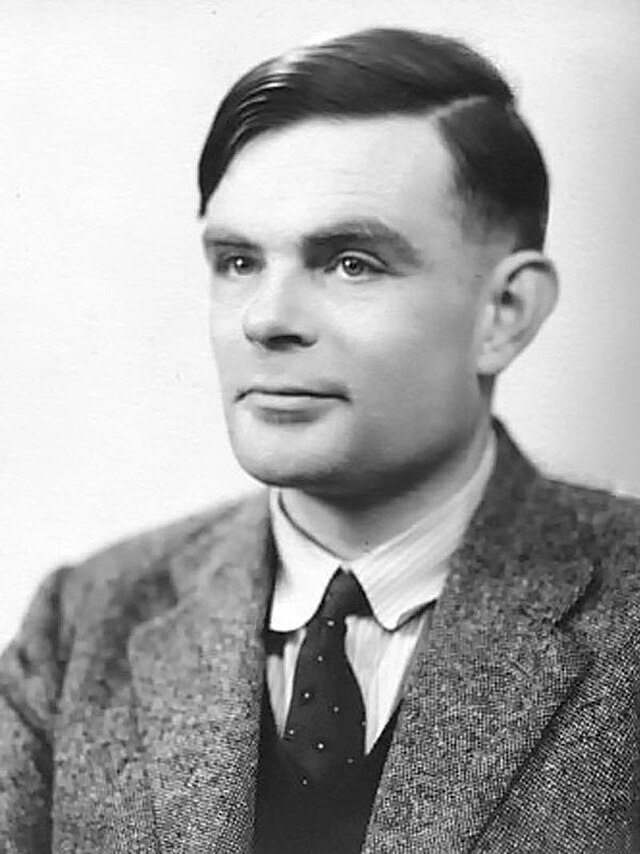
\includegraphics[width=7cm]{./pictures/Alan_Turing.jpg}
	\caption{Alan Turing}
	\label{Turing}
\end{figure} 

\textsc{Alan Turing} (1912--1954) az 1930-as évek elején megalkotta a Turing-gépet \textsc{Kurt Gödel} (1906--1978) munkássága alapján, amely a modern számítógépek elméleti alapját képezte. 1950-ben publikálta a ''Computing Machinery and Intelligence'' című tanulmányát, amelyben felvetette a gépek gondolkodási képességének kérdését, és bevezette a híres Turing-tesztet, amely azt vizsgálja, hogy egy gép képes-e emberihez hasonló intelligens viselkedésre. \cite{AlanTuring,CMI}

\textsc{John McCarthy} (1927–-2011) amerikai számítástechnikai és kognitív tudós volt, akit a mesterséges intelligencia egyik alapítójaként tartanak számon. Ő alkotta meg a "mesterséges intelligencia" (artificial intelligence) kifejezést az 1956-os Dartmouth Konferencián, amelyet ő szervezett, és amelyet az MI hivatalos születésnapjaként tartanak számon. McCarthy 1958-ban kifejlesztette a Lisp programozási nyelvet, amely a mesterséges intelligencia-kutatás egyik legfontosabb eszközévé vált. Emellett jelentős hatással volt az ALGOL nyelv tervezésére, népszerűsítette az időosztásos rendszereket, és feltalálta a szemétgyűjtést (garbage collection). 

\begin{figure}[h!]
	\centering
	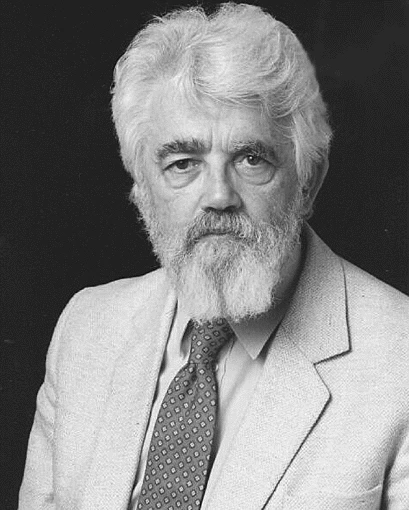
\includegraphics[width=5cm]{./pictures/John_McCarthy.png}
	\caption{John McCarthy}
	\label{McCarthy}
\end{figure}

McCarthy munkássága jelentős hatással volt a mesterséges intelligencia fejlődésére. Az 1960-as és 1970-es években az MI-kutatás optimizmusa után nehéz időszak jött, amikor a fejlődés lelassult a korlátozott számítási kapacitás és a finanszírozási problémák miatt. Azonban McCarthy és kortársai kitartása hozzájárult ahhoz, hogy az MI napjainkban az egyik legdinamikusabban fejlődő területté váljon. Az utóbbi évtizedekben a gépi tanulás, a neurális hálózatok és a mélytanulás forradalmasították az MI-t, amely ma már számos területen, például az orvostudományban, az iparban és az önvezető autókban is kulcsszerepet játszik. \cite{JohnMcCarthy}

\section{Játékelmélet}

A játékelmélet a matematika egyik, tudományágak közé egyértelműen nehezen besorolható (interdiszciplináris) ága, mely olyan kérdésekkel foglalkozik, hogy mi az ésszerű (racionális) viselkedés olyan helyzetekben, ahol minden résztvevő döntéseinek eredményét befolyásolja a többi résztvevő lehetséges választásai, röviden a stratégiai problémák elmélete. A játékelmélet alapjait Neumann János fektette le ''Zur Theorie der Gesellschaftsspiele'' című 1928-as munkájában \cite{Neumann}, majd Oskar Morgenstern neoklasszikus matematikus-közgazdásszal közösen megírta a „Játékelmélet és gazdasági viselkedés” című (The Theory of Games and Economic Behavior, 1944) művüket. \cite{Jatekelmelet,JatekelmeletEn} Ezen művek alapján a következő fogalmakat tisztáznunk kell \cite{NeumannOskar}:

\begin{itemize}
	\item A \emph{játék} a játékosok viselkedését és lényeges körülményeket meghatározó szabálysor által leírt folyamat.
	\item Az információs halmaz (ismeret) meghatározó szerepű. Ez azt jelenti, hogy az információs halmaz alapján különböző típusokat sorolhatunk fel, például a \emph{tökéletes információs} és \emph{véges}, ahol minden résztvevő birtokolja az összes vonatkozó adatot (szabályok, lehetséges és korábbi események).
	\item Egy játék lehet két- vagy többszemélyes.
	\item Mikor a játékban a játékosok versengenek egymással, akkor \emph{nem kooperatív} játékról beszélünk.
	\item Zérusösszegű az a játék, amelyben a játékosok csak az ellenfelük nyereségük csökkentésével növelhetik nyereségüket.
	\item A játékost győzelemre, de minimum döntetlenre segítő módszere a \emph{stratégia}. Ilyenkor kihasználhatja az ellenfél érzékelt hibáit.
\end{itemize} 



\subsection{Minimax algoritmus}

A minimax elv olyan alkalmazott döntési szabály a játékelméletben, ami szerint azt a lehetőséget kell választani, ami minimalizálja a maximális veszteséget. Ezt az elvet felhasználhatjuk a kétfős zérusösszegű játékoknál, ami magába foglalja a két játékos szimultán döntéseit és a felváltva tett lépéseit is. \cite{MiniMaxEnWiki}

Formális definíció szerint a következőképpen tudjuk felírni a számítást:

\begin{equation*}
\overline{v_{i}}=\underset{{a_{-i}}}{\min} \underset{{a_{i}}}{\max} v_{i}(a_{i}, a_{-i})
\end{equation*}

A minimax érték azt fejezi ki, hogy egy játékos legrosszabb esetben mekkora értéket érhet el, ha a többi játékos a számára legkedvezőtlenebb stratégiát követi. Másképpen megfogalmazva, ez az a legnagyobb érték, amelyet a játékos garantáltan megszerezhet, ha ismeri a többi játékos lépéseit. 

Egy kétszemélyes játékban az egyik játékos a maximalizáló, aki a saját pontszámának maximalizálására törekszik, míg a másik a minimalizáló, aki a maximalizáló pontszámának minimalizálására törekszik. Az algoritmus úgy működik, hogy kiértékeli az összes lehetséges lépést mindkét játékos számára, előrejelzi az ellenfél válaszait, és kiválasztja az optimális lépést annak érdekében, hogy a lehető legjobb eredményt biztosítsa. \cite{MiniMaxGfG}

\subsection{Minimax alfa-béta vágással}

\chapter{Implementáció}

\section{Technológiák}

\subsection{Játékmotor}

A szakdolgozatom megvalósításához a Unity-t (korábban Unity3D) használom. A Unity egy világszerte ismert és használt videójáték-motor, amelyet a Unity Technologies fejleszt 2005 óta. A motor támogat több különböző platformot, például PC, videójáték konzolok és okostelefonok. Különösen kedvelik a kezdő játékfejlesztők a letisztult felülete és egyszerű használata miatt. Választásom azért esett a Unity-re, mert a szkriptekhez natívan támogatja a C\# nyelvet. A szakdolgozatomban a Unity-nek a 2022.3.32f1-es verzióját használom.

\begin{figure}[h!]
	\centering
	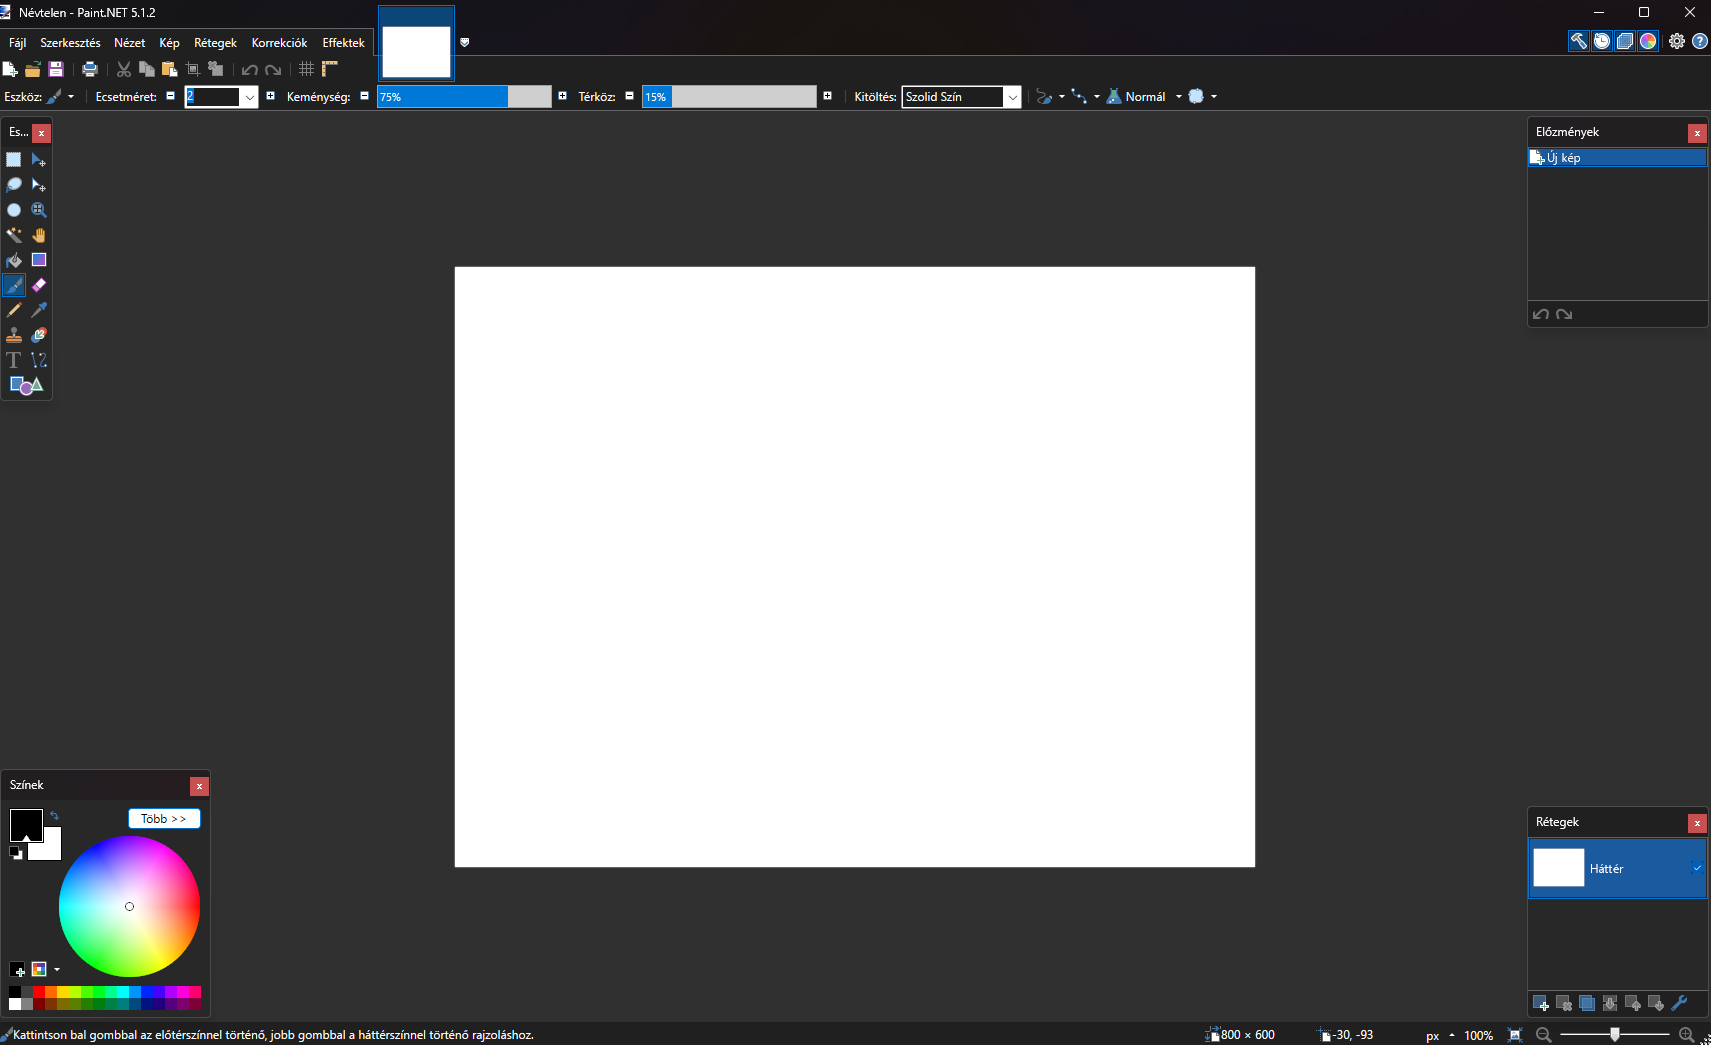
\includegraphics[width=15cm]{./pictures/paint_net.png}
	\caption{Paint.NET felülete}
	\label{PaintNET}
\end{figure}

\subsection{Grafikus szerkesztő}

A szakdolgozatomat a Unity-be beépített színeken és objektumokon kívül, általam készített pixelábrákat használok a karakterek képeként, amelyekhez a Paint.NET szoftvert használtam. A Paint.NET egy szabad licenszű, rasztergrafikus alkalmazás, amelyet a dotPDN fejleszt. A szakdolgozatom készítésekor 5.1.2 verzióját használtam a szoftvernek.

\section{Megjelenítés}

A játék készítésekor törekedtem a minimalista és könnyen vezérelhető kezelőfelületre. A Unity-ben úgynevezett \emph{scene}-ekre lehet osztani az játékot, legközelebbi példaként a \emph{WinForms} alkalmazásokban egy új \emph{form} létrehozásával lehet párhuzamba hozni ezt a megoldást. A játékom három scene-ből áll: \textbf{MenuScene}, \textbf{GameScene} és \textbf{EndScene}.

\subsection{MenuScene}

\begin{figure}[h!]
	\centering
	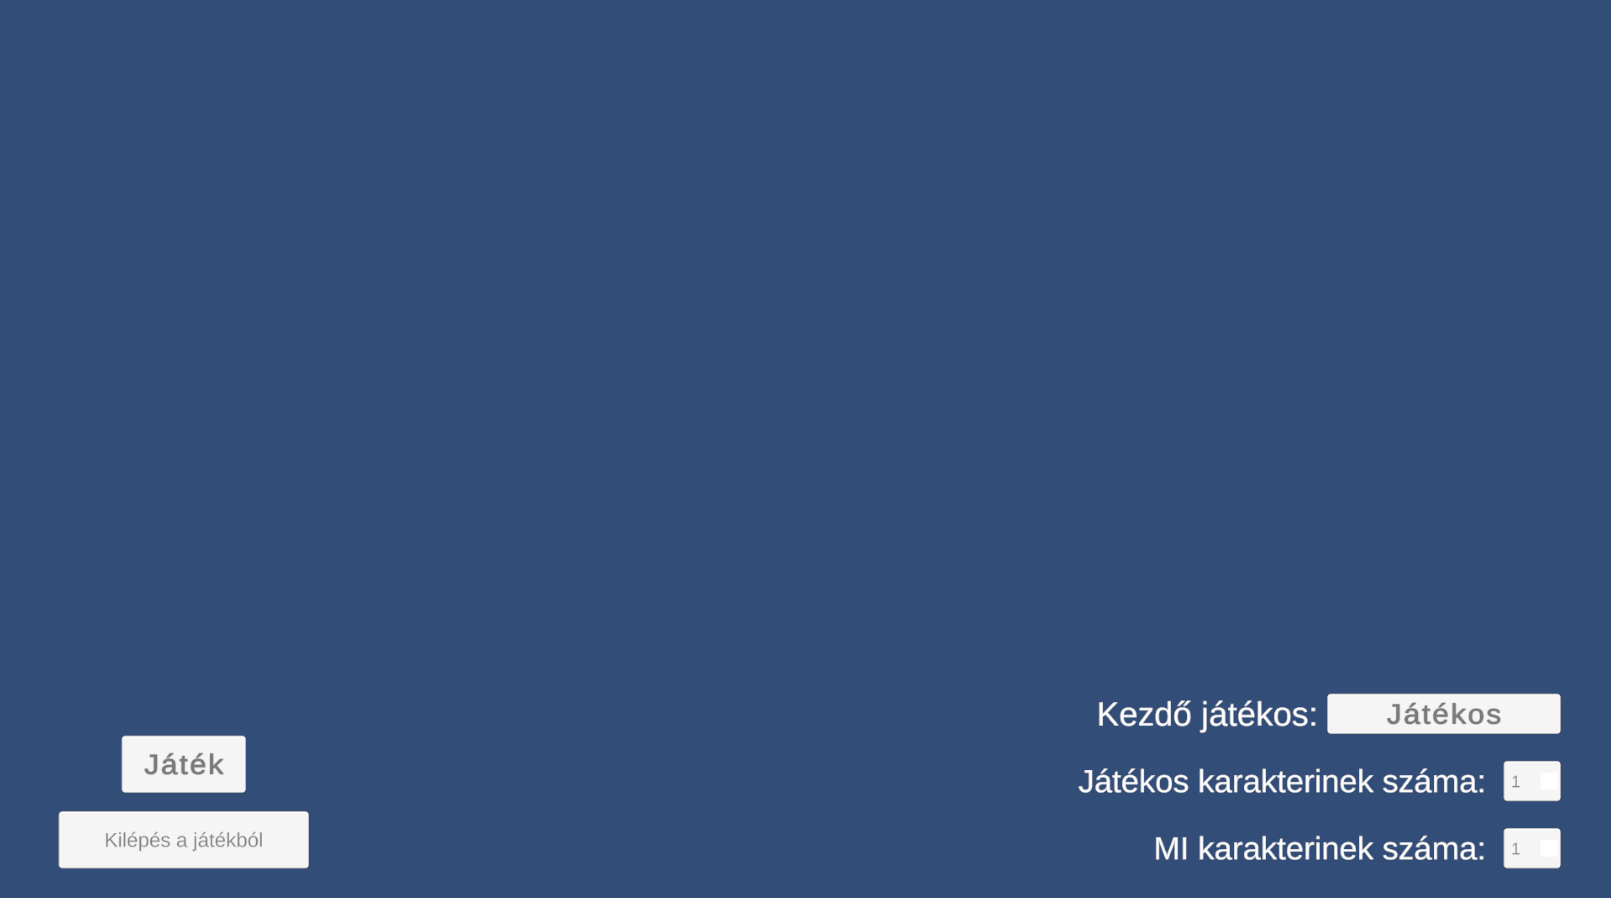
\includegraphics[width=15cm]{./pictures/game_menu.png}
	\caption{A játék menüjének felépítése}
	\label{menuscene}
\end{figure}

A \emph{MenuScene} az alap \emph{Camera} objektumon kívül tartalmaz egy \emph{Canvas} 2D-s objektumot. Ezen a felületen találhatóak a különböző funkciókat betöltő objektumok, a kép bal alsó sarkában található az \emph{ExitButton} nevű gomb objektum, amely névéhez illően kilép az alkalmazásból, felette található a \emph{PlayButton} gomb, amely a felhasználó által kiválasztott beállítások alapján elindítja a játékot. A képernyő jobb oldalán lehet találni a beállításokat módosító gombokat és karakterek számát kiválasztó \emph{Dropdown} listák. A gomb megnyomásával kiválaszthatja a játékos, hogy Önmaga szeretné kezdeni a játékot vagy átadja a kezdés jogát a gépnek. A listákban a játékos ki tudja választani, hogy hány karakterrel induljon a játék, amely a korábban \aref{rules} szekcióban említett szabályok alapján egytől négy karakterig lehetséges. A \emph{MenuScene} felépítése \aref{menuscene} ábrán látható.

\subsection{GameScene}

A \emph{GameScene} a szakdolgozatom fénypontja, az alkalmazás magja. A scene tartalmaz kettő objektumot: \emph{GridObjectPrefab} nevű \emph{prefab}-et és egy canvas-t. 

A \emph{prefab} \emph{GameObject}-ek egyvelege, amelyben a programozó tárolhat konfigurációt, mező értékeket illetve gyermek GameObject-eket. Természetesen ezeket újra fel lehet használni, akár kódból példányosítani, illetve törölni is lehet őket a scene-ből. \cite{UnityDocsPrefab} 

Ebben a prefab-ben található a későbbi \ref{state} szekcióban tárgyalt állapottér megjelenítése, amelynek reprezentációs mátrixát egy \emph{Grid} objektummal implementálom. A grid objektum magában még nem a megjelenítést oldja meg, csupán a mátrix értékeit adom át a komponensnek átalakítva, ehhez még szükséges úgynevezett \emph{Tileset} objektumot létrehoznom. Ez a tileset objektum \emph{Tile} objektumokból áll, ami pedig kétféle négyzet 2D-s \emph{sprite} felületet vehet fel, ez függ a koordinátájától, így sakktábla (\ref{gamegrid}~ábra) hatást keltve jelenik meg. 

\begin{figure}[h!]
	\centering
	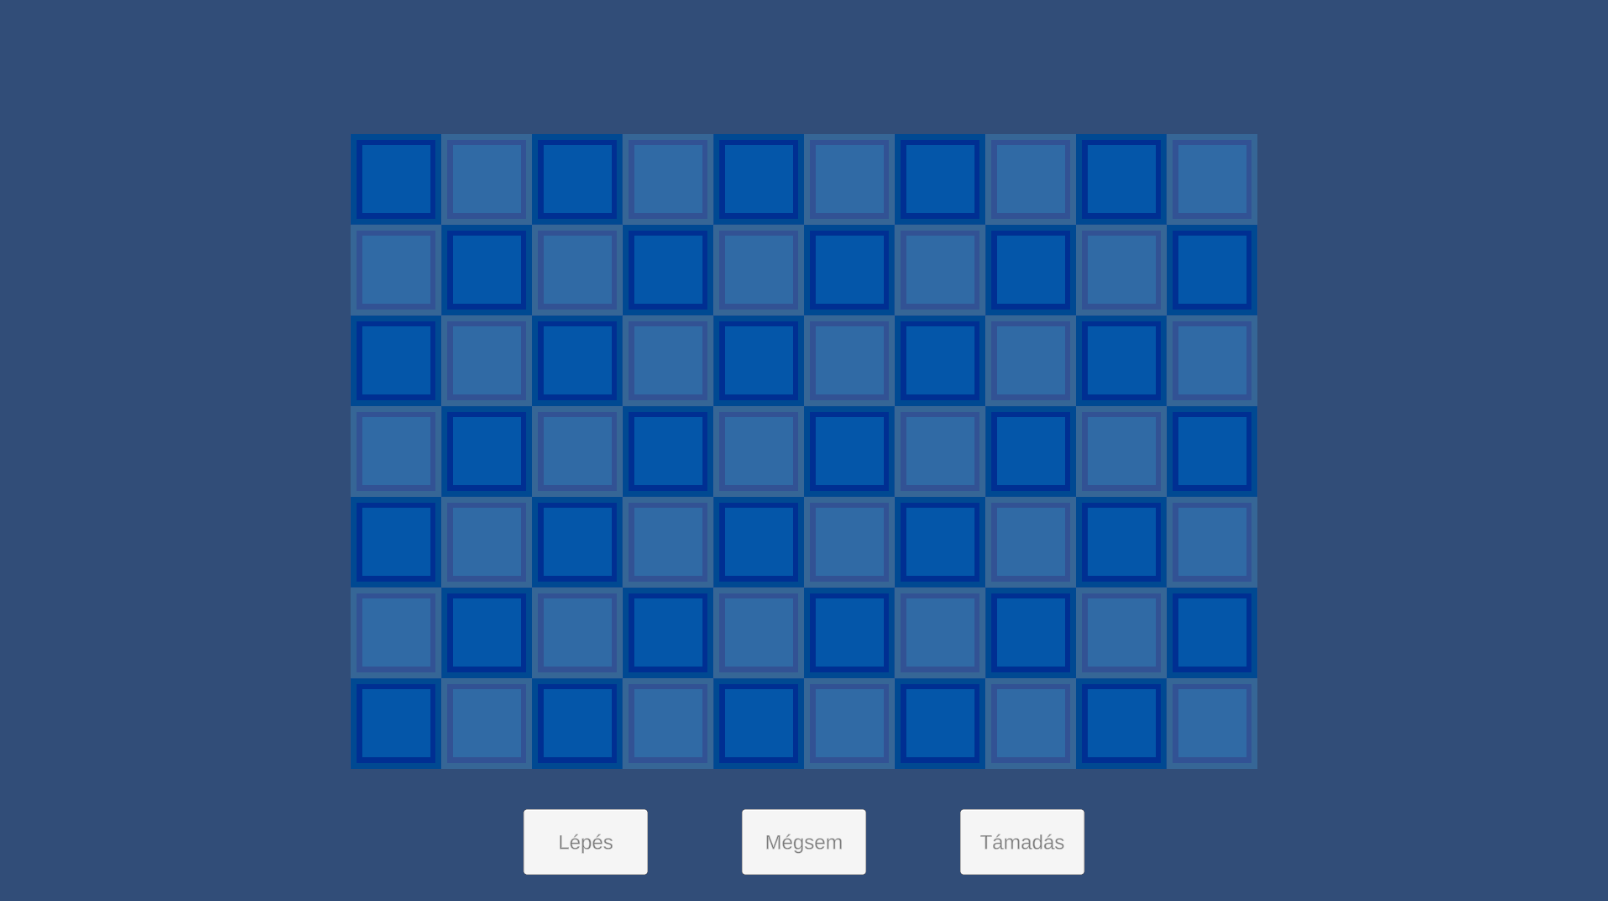
\includegraphics[width=15cm]{./pictures/game_grid.png}
	\caption{A játéktábla karakterek nélkül}
	\label{gamegrid}
\end{figure}

A játék indulása során az állapottérből lekérdezett pozíciók alapján ezen prefab gyermekobjektumaként példányosítom a játékos és MI karakterek prefab-jeit. Ezek a prefab-ek tárolják magukban az állapottérben is tárolt adatokat (név, életerő, pozíció), illetve a karakter tulajdonosától függő sprite-ot.

A játék ideje alatt, ahogyan a karakterekkel lépnénk vagy támadnánk, a szabályoknak megfelelő módon a végrehajtható művelet céljának négyzete zöld színt kap, amennyiben ez nem lehetséges, piros színt kap árnyalatnak (\ref{gamemove}~ábra). Amikor a játékos a felületen kurzorát mozgatja művelet kiválasztása nélkül, a négyzet, amelyen a kurzor található, szürke árnyalatot kap.

\begin{figure}[h!]
	\centering
	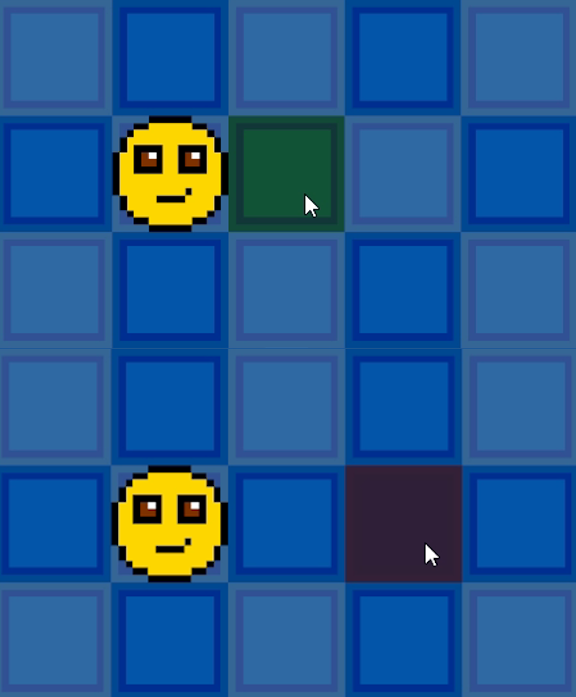
\includegraphics[width=6cm]{./pictures/game_move_tile.png}
	\caption{Példa helyes és helytelen lépésre}
	\label{gamemove}
\end{figure}


\section{Állapottér} \label{state}

\section{Operátor} \label{operator}

\section{Operátorok felépítése} \label{operatorbuild}

\section{Operátor generálás} \label{operatorgen}

\section{Minimax} \label{minimax}

\section{Minimax alfa-béta vágással} \label{minimaxalphabeta}

\section{Heurisztika} \label{heuristics}


\chapter{Tesztelés}

\section{Manuális tesztelés}

\chapter*{Összegzés}
\addcontentsline{toc}{chapter}{Összegzés}


\begin{thebibliography}{2}
\addcontentsline{toc}{chapter}{\bibname}

\bibitem{Persona}
\textsc{Wikipédia:} \emph{Persona (series)} 
\url{https://en.wikipedia.org/wiki/Persona_(series)}, Megtekintés dátuma: 2025.03.19.

\bibitem{Persona3}
\textsc{Wikipédia:} \emph{Persona 3 Reload} 
\url{https://en.wikipedia.org/wiki/Persona_3_Reload}, Megtekintés dátuma: 2025.03.19.

\bibitem{Persona1}
\textsc{Wikipédia:} \emph{Revelations:~Persona} 
\url{https://en.wikipedia.org/wiki/Revelations:_Persona}, Megtekintés dátuma: 2025.03.19.

\bibitem{Persona1Gameplay}
\textsc{YouTube:} \emph{Persona: Mastering the Formation System} 
\url{https://www.youtube.com/watch?v=t_FPK84jcbE}, Megtekintés dátuma: 2025.03.19.

\bibitem{AlanTuring}
\textsc{Wikipédia:} \emph{Alan Turing} 
\url{https://en.wikipedia.org/wiki/Alan_Turing}, Megtekintés dátuma: 2025.03.19.

\bibitem{CMI}
\textsc{Wikipédia:} \emph{Computing Machinery and Intelligence} 
\url{https://en.wikipedia.org/wiki/Computing_Machinery_and_Intelligence}, Megtekintés dátuma: 2025.03.19.

\bibitem{JohnMcCarthy}
\textsc{Wikipédia:} \emph{John McCarthy (computer scientist)} 
\url{https://en.wikipedia.org/wiki/John_McCarthy_(computer_scientist)}, Megtekintés dátuma: 2025.03.19.

\bibitem{Neumann}
\textsc{Neumann János}: \emph{On the theory of games of strategy}, Sonnya Bargmann fordítása, 1928.
\url{https://cs.uwaterloo.ca/%7Ey328yu/classics/vonNeumann.pdf}, Megtekintés dátuma: 2025.03.19.

\bibitem{Jatekelmelet}
\textsc{Wikipédia:} \emph{Játékelmélet} 
\url{https://hu.wikipedia.org/wiki/J%C3%A1t%C3%A9kelm%C3%A9let}, Megtekintés dátuma: 2025.03.19.

\bibitem{JatekelmeletEn}
\textsc{Wikipédia:} \emph{Game theory} 
\url{https://en.wikipedia.org/wiki/Game_theory}, Megtekintés dátuma: 2025.03.19.

\bibitem{NeumannOskar}
\textsc{Neumann János, Oskar Morgenstern}: \emph{Theory of Games and Economic Behavior}, 1944.
\url{https://archive.org/details/in.ernet.dli.2015.215284/page/n5/mode/2up}, Megtekintés dátuma: 2025.03.19.


\bibitem{MiniMaxEnWiki}
\textsc{Wikipédia}: \emph{Minimax} 
\url{https://en.wikipedia.org/wiki/Minimax}, Megtekintés dátuma: 2025.03.19.

\bibitem{MiniMaxGfG}
\textsc{GeeksforGeeks}: \emph{Mini-Max Algorithm in Artificial Intelligence} 
\url{https://www.geeksforgeeks.org/mini-max-algorithm-in-artificial-intelligence/}, Megtekintés dátuma: 2025.03.19.

\bibitem{UnityDocsPrefab}
\textsc{Unity Documentation}: \emph{Prefabs} 
\url{https://docs.unity3d.com/2022.3/Documentation/Manual/Prefabs.html/}, Megtekintés dátuma: 2025.03.26.
\end{thebibliography}

% Aláírt, szkennelt nyilatkozat beillesztése a szakdolgozat végére
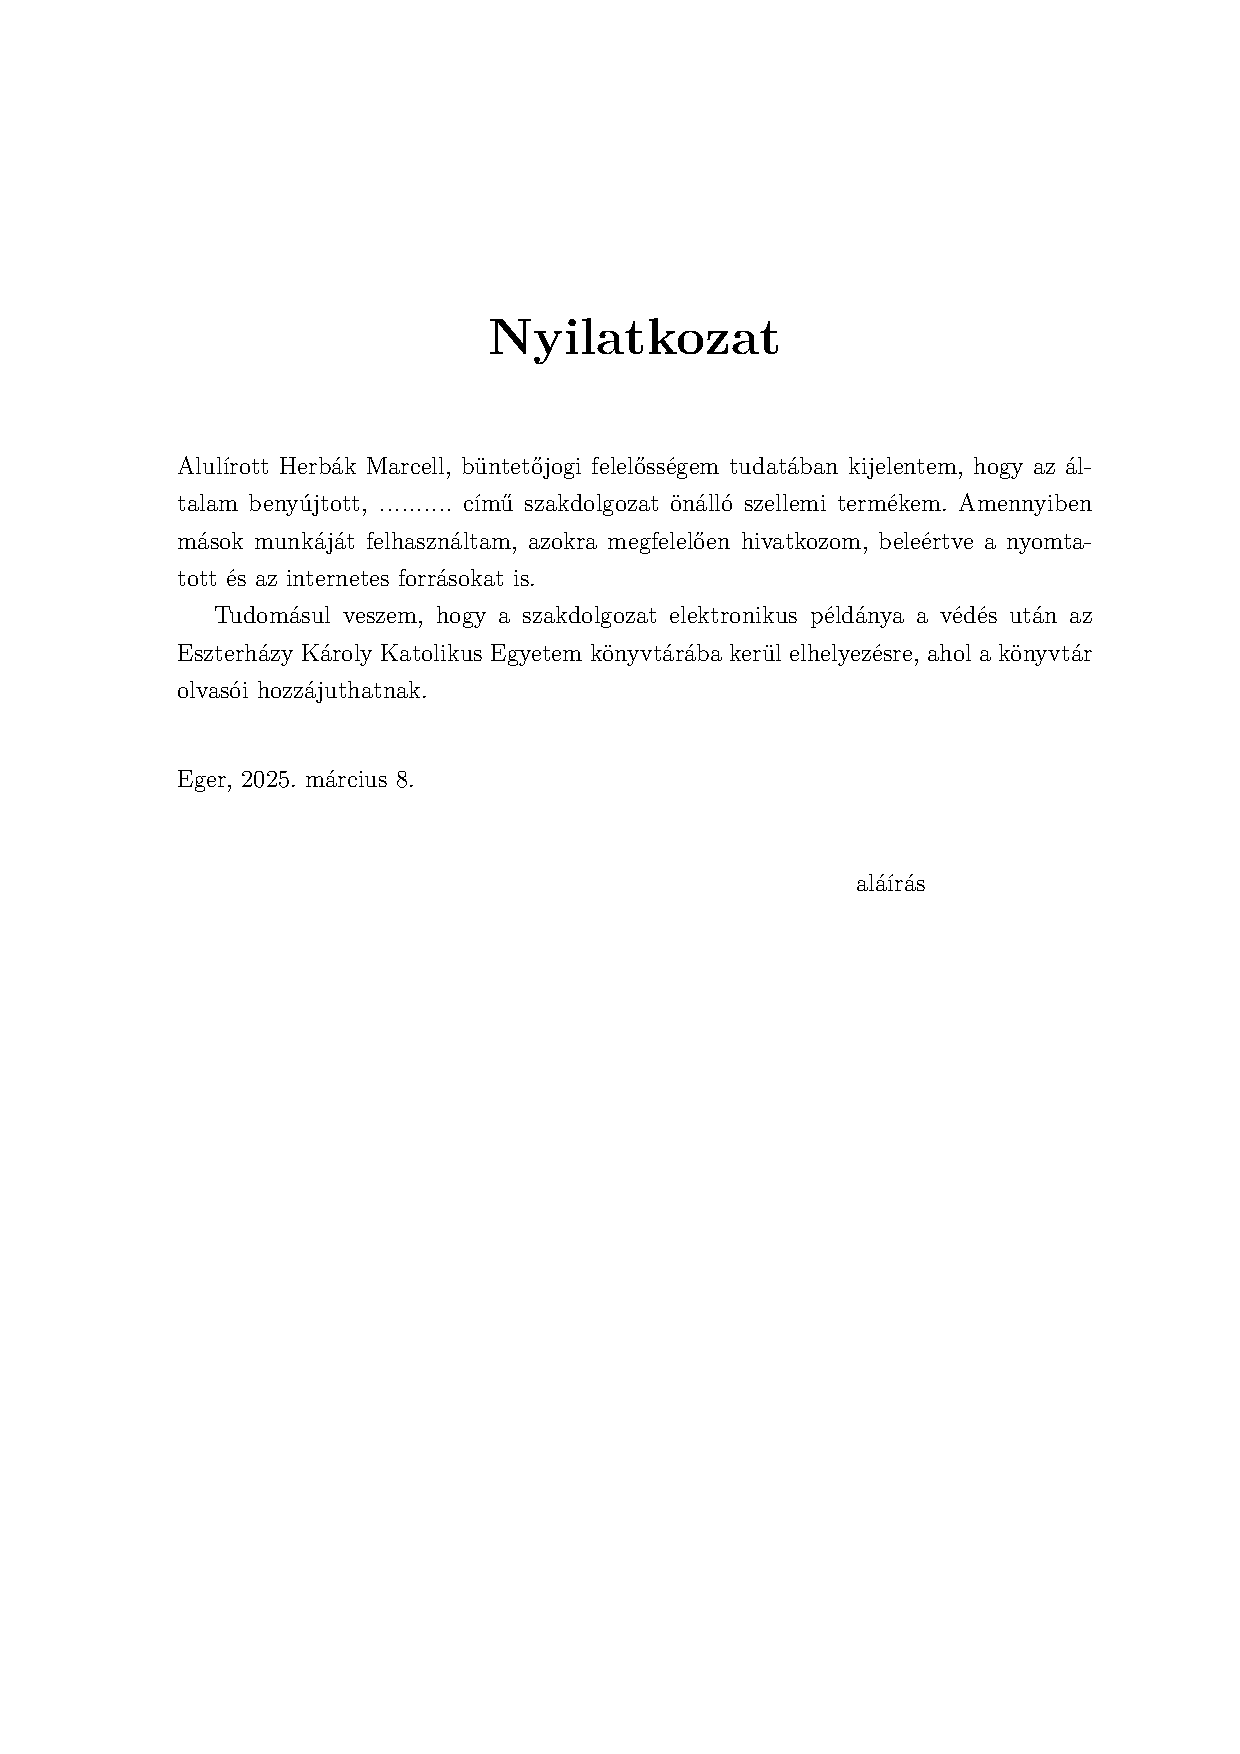
\includepdf{nyilatkozat/nyilatkozat.pdf}
\end{document}